%% cuts.tex --- text removed from main.tex, kept for the record.
%%
%% THIS FILE IS NOT \input BY main.tex. It does not compile on its own and is
%% not meant to. It is an archive, so that nothing below has to be
%% reconstructed from git if we change our minds.
%%
%% ---------------------------------------------------------------------------
%% 2026-08-31: ChangeRoot and PruneDownTo removed.
%% ---------------------------------------------------------------------------
%%
%% AM's call, from the pen-and-paper read of 2026-08-31, recorded as item 3 of
%% paper/pen-notes-buckets.md: "I am strongly considering removing ChangeRoot
%% and PruneDownTo. No reader will read this paper sans those and then say
%% 'hey, where are those?'"
%%
%% What the cut costs, checked before it was made:
%%
%%   Nothing in the completeness argument. sec:fallback's always-available plan
%%   is Replace([], p_2), which expands to Designate, Quiesce, and Undesignate.
%%   Neither ChangeRoot nor PruneDownTo is needed to reach any p_2 from any p_1,
%%   so no theorem weakens. The grammar goes from seven forms to six and the
%%   idiom set from four to three.
%%
%%   One thing in section 8. port_root was justified there entirely by
%%   ChangeRoot ("This port_root state is what makes ChangeRoot expressible").
%%   The wrapper itself was left in place, since it may still be wanted for
%%   port multiplexing, but it now has no stated reason to exist. An \xxx in
%%   main.tex flags that for Zhiyuan. See region 15 below.
%%
%% To restore: the regions below are verbatim and in document order, each with
%% the place it came from. Regions 1 through 6 and 8, 9, 11, 13, 14, 15 are
%% fragments spliced into surviving prose; regions 7, 10, 12, and 16 are whole
%% units that can be pasted back where their headers say.
%%
%% ===========================================================================


% ---------------------------------------------------------------------------
% 1. Preamble macros
% From: main.tex preamble
% ---------------------------------------------------------------------------

\newcommand{\ChangeRoot}{\textsf{ChangeRoot}}
\newcommand{\PruneDownTo}{\textsf{PruneDownTo}}


% ---------------------------------------------------------------------------
% 2. The grammar production
% From: fig:delta-grammar, \S4.1
% ---------------------------------------------------------------------------

\mid & \ChangeRoot(\mathit{path})\\[6pt]


% ---------------------------------------------------------------------------
% 3. The edit-site exception
% From: \S4.1, just before fig:delta-grammar
% ---------------------------------------------------------------------------

The node a form's \pth names is its \emph{edit site}, with \ChangeRoot{} the one exception, since there the path gives the surviving subtree instead.


% ---------------------------------------------------------------------------
% 4. The idiom one-liner
% From: \S4.1, after the not-in-the-grammar paragraph
% ---------------------------------------------------------------------------

\Retire{} drains a subtree and then removes it, \Replace{} swaps one subtree for another in place, and \PruneDownTo{} discards everything except a chosen subtree.


% ---------------------------------------------------------------------------
% 5. The completeness clause
% From: \S4.1, third of the three properties
% ---------------------------------------------------------------------------

And they are \emph{complete}, since the seven together reach any \(p_2\) from any \(p_1\), which \cref{sec:fallback} shows by exhibiting a sequence that always works.


% ---------------------------------------------------------------------------
% 6. The fig:delta-semantics row
% From: fig:delta-semantics, \S4.3
% ---------------------------------------------------------------------------

\ChangeRoot(\nu) & C@\nu & p \mapsto p@\nu


% ---------------------------------------------------------------------------
% 7. \S4.3.7 in full
% From: the whole subsubsection, sec:changeroot
% ---------------------------------------------------------------------------

\subsubsection{\texorpdfstring{\(\ChangeRoot(\nu)\)}{ChangeRoot}}\label{sec:changeroot}
% nu looks like v and looks confusing. Change to a different letter. 

% I am strongly considering removing ChangeRoot and PruneDownTo. No reader will read this paper sans those and then say "hey, where are those?"

\(\nu : \mathit{path}\) is the subtree promoted to the new root; \ChangeRoot{} discards every ancestor above \(C@\nu\).
It is the only form that erases structural ancestors; the mechanics are short but the Notes below are substantive.

\paragraph{Definition}

\ChangeRoot{} is defined when \(\nu\) is non-empty, resolves in \(C\), and every node strictly above \(C@\nu\) is \emph{unary} with its sole arm continuing toward \(C@\nu\), so that the discarded chain carries no off-path traffic.
\(C@\nu\) and its subtree are kept unchanged; every proper ancestor's \((\mathit{state}, \mathit{pifo}, \mathit{z})\) is discarded.

\paragraph{Pol-level reading}

The promoted subtree becomes the root, and a root has no parent to annotate it, so the metadatum it carried is discarded along with the ancestors that read it.

\paragraph{Notes}

\emph{Why the unary precondition.}
The precondition rules out, by construction, any silently-dropped packet-bearing siblings.
A non-unary ancestor would have arms branching off the path to \(C@\nu\); those subtrees would vanish with their ancestor, taking their packets with them.
Allowing this would make \ChangeRoot{} a structural deletion of arbitrarily many off-path subtrees masquerading as a root change, with no semantic story for those packets.
An operator may still want to prune to a subtree whose ancestor chain branches off into packet-bearing relatives.
That is the \PruneDownTo{} idiom, which drains and \Remove{}s those siblings in sequence.
Doing so reduces the chain above \(C@\nu\) to the unary shape that \ChangeRoot{} accepts.

\emph{What the chain carries, and what is discarded.}
An internal node's \nodestate, rank function, and \pifo ordering exist to pick among siblings.
A unary node has no siblings to choose between.
Every pop is forced into its one arm.

What can remain active at a unary node is rank computation that depends on per-packet attributes rather than on sibling identity.
If a chain's disciplines do no such per-packet reordering, each unary node along the chain is operationally a passthrough, and the non-disruption argument above extends to every subsequent pop and push.
If they do, the chain is actively shaping traffic, and \ChangeRoot{} removes that shaping.
LSTF~\cite{Mittal16} is a canonical example, ranking each packet by its deadline.
It is not one of our three instantiated disciplines, but it is the kind of discipline the open family of \cref{sec:policy-dsl} admits.
That is precisely the form's intended role.
It is the atomic step by which the operator says ``promote \(p@\nu\) to the root and discard the ancestor shaping above it.''
\PruneDownTo{} packages this with the upstream draining and \Remove{}s that make the chain unary in the first place, so the operator's request (``prune to this subtree'') is realized as a sequence whose final step discards exactly the ancestor influence that the operator has chosen to abandon.

\emph{Pol-level effect.}
The \pol changes from the unary chain wrapping \(p@\nu\), for instance \(\Strict(p@\nu)\), to just \(p@\nu\).
This is \pol-visible: the root discipline observably changes, which is the substantive content of the form.
Whether that pol-visible change reorders in-flight traffic depends on whether the discarded chain was doing per-packet reordering (see previous Note).


% ---------------------------------------------------------------------------
% 8. \S5.2's clause in the \xxx to Adrian
% From: sec:nondisruption
% ---------------------------------------------------------------------------

My counter-offer is to promote non-disruption to a collected theorem rather than demote it: every \(\delta\) leaves the \pop{} sequence unchanged, which is what the \Designate, \Undesignate, and \ChangeRoot{} arguments actually establish and what the current per-form wording understates.}


% ---------------------------------------------------------------------------
% 9. \S5.2's counting sentences
% From: sec:nondisruption
% ---------------------------------------------------------------------------

Four of the seven pass that check outright.
\Designate{} inserts a node whose \pifo is not empty, \Undesignate{} drops one, and \ChangeRoot{} discards a whole chain of them, so those three need an argument of their own.


% ---------------------------------------------------------------------------
% 10. \S5.3.5 in full
% From: the whole subsubsection
% ---------------------------------------------------------------------------

\subsubsection{\texorpdfstring{\(\ChangeRoot(\nu)\)}{ChangeRoot}}

\paragraph{Characterization}
\(\lfloor \cdot \rfloor\) is a structural recursion, so it commutes with subtree projection: \(\lfloor C@\nu \rfloor = p \mathbin{@} \nu\), giving \(p' \eqR \psem{\ChangeRoot(\nu)}(p)\).

\paragraph{Preservation and non-disruption}

\emph{Preservation of \(\vdash\).} \(\vdash C\) is a conjunction of per-node obligations, and those on \(C@\nu\)'s nodes are exactly \(\vdash C@\nu = \vdash C'\).
The discarded ancestors' obligations are forgotten with them.
\emph{Non-disruption.} Every in-flight packet sits in a \pifo within \(C@\nu\) (the discarded ancestor pifos held routing entries, not packets).
Those entries are redundant.
A \pop{} before \(\delta\) descends the unary chain, and each ancestor pifo has the single slot \(0\), so every such pop is forced to slot \(0\) and lands at \(C@\nu\).
A \pop{} after \(\delta\) acts on \(C@\nu\) directly and returns the same packet.
So \ChangeRoot{} is non-disruptive.


% ---------------------------------------------------------------------------
% 11. The PruneDownTo idiom definition
% From: fig:gseq-idioms, \S6.2
% ---------------------------------------------------------------------------

\PruneDownTo(\mathit{path}) \;=\;\\
\quad \Retire(\pi_a)\,;\, \ldots\,;\, \Retire(\pi_z)\,;\, (\mathtt{true};\, \ChangeRoot(\mathit{path}))


% ---------------------------------------------------------------------------
% 12. \S6.2's PruneDownTo bullet in full
% From: including the A(B(D(F,G),E),C) example and its path table
% ---------------------------------------------------------------------------

\item \textbf{\PruneDownTo(\pth)} retires every off-path subtree along the route from the root to \pth (call them \(\pi_a, \ldots, \pi_z\)), then \ChangeRoot{}s to \pth.
This idiom is the operator-facing way to say ``abandon everything except this subtree.''

Each \Retire{} removes one off-path subtree; once they have all fired, every ancestor along the path is unary, satisfying \ChangeRoot's precondition (\cref{sec:changeroot}).
The \Retire{}s on disjoint off-path subtrees commute, so any ordering suffices; we use root-first as a stable convention.

For instance, suppose the running tree is \(A(B(D(F,\allowbreak G), E),\allowbreak C)\), with edges labeled by the parent-side index:

\begin{center}
\begin{minipage}{0.55\linewidth}
\centering
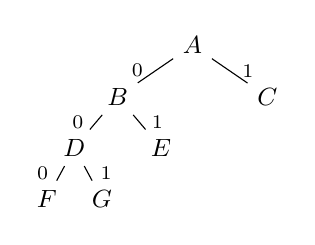
\begin{tikzpicture}[
  level distance=0.65cm,
  level 1/.style={sibling distance=1.9cm},
  level 2/.style={sibling distance=1.1cm},
  level 3/.style={sibling distance=0.7cm},
  every node/.style={font=\small},
  edge from parent/.style={draw},
  every child/.style={font=\scriptsize}
]
\node {\(A\)}
  child {node {\(B\)}
    child {node {\(D\)}
      child {node {\(F\)} edge from parent node[left, xshift=-1pt] {\scriptsize 0}}
      child {node {\(G\)} edge from parent node[right, xshift=1pt] {\scriptsize 1}}
      edge from parent node[left, xshift=-1pt] {\scriptsize 0}
    }
    child {node {\(E\)} edge from parent node[right, xshift=1pt] {\scriptsize 1}}
    edge from parent node[left, xshift=-1pt] {\scriptsize 0}
  }
  child {node {\(C\)} edge from parent node[right, xshift=1pt] {\scriptsize 1}};
\end{tikzpicture}
\end{minipage}%
\begin{minipage}{0.35\linewidth}
\centering
\small
\begin{tabular}{@{}l@{\quad}l@{}}
\(A\) & \([\,]\) \\
\(B\) & \([0]\) \\
\(C\) & \([1]\) \\
\(D\) & \([0,0]\) \\
\(E\) & \([0,1]\) \\
\(F\) & \([0,0,0]\) \\
\(G\) & \([0,0,1]\) \\
\end{tabular}
\end{minipage}
\end{center}
The operator wants to retain only \(E\), so they issue \PruneDownTo(\([0,1]\)).
The off-path subtrees are \(D(F, G)\) (at \([0,0]\)) and \(C\) (at \([1]\)).
So \PruneDownTo(\([0,1]\)) expands to \Retire(\([0,0]\)) ; \Retire(\([1]\)) ; (\(\mathtt{true}\); \ChangeRoot(\([0,0]\))).

The path \([0,0]\) appears twice in this expansion with different referents.
In \Retire(\([0,0]\)) it points to \(D(F, G)\), the operand at the moment that \Retire{} fires.
In the final \ChangeRoot(\([0,0]\)) it points to \(E\), which moved from \([0,1]\) to \([0,0]\) once \(D(F, G)\) was retired.
A path-resolution system computes these targets automatically at idiom expansion; the operator only writes \PruneDownTo(\([0,1]\)), naming \(E\) by its location at the moment of request.


% ---------------------------------------------------------------------------
% 13. \S6.2's opposite-move opening
% From: the two sentences that framed the paragraph against PruneDownTo
% ---------------------------------------------------------------------------

\emph{The opposite move.}
\PruneDownTo{} keeps one subtree and abandons everything around it.
The opposite move would keep the running tree and splice fresh structure \emph{above and around} it, with the running root becoming a child of a newly introduced context.


% ---------------------------------------------------------------------------
% 14. The planner's second case
% From: \S7.2's top-level pass
% ---------------------------------------------------------------------------

\item \(p_2\) embeds in \(p_1\) at \pth. Emit \(\PruneDownTo(\mathit{path})\).
A structural sub-policy test walks \(p_1\) looking for a subtree equal to \(p_2\); if it finds one, \pth names where it sits.
The match is unique: by \cref{sec:policy-dsl}'s leaf-partition validity each flow in \(p_2\) may appear at most once in \(p_1\), so \(p_1\) can host \(p_2\) as a subtree in at most one position.
This test runs only at the top level.


% ---------------------------------------------------------------------------
% 15. \S8.2's port_root justification
% From: the two sentences naming ChangeRoot
% ---------------------------------------------------------------------------

This \texttt{port\_root} state is what makes \ChangeRoot{} expressible, and it is maintained by two complementary mechanisms.
On every form except \ChangeRoot, the \texttt{walk(...)} calls that touch \texttt{Assoc}/\texttt{Map} start at \texttt{port\_root} and so update its tables in lockstep with the actual root's.
On \ChangeRoot, the lowering issues no flow-table writes against \texttt{port\_root} at all.


% ---------------------------------------------------------------------------
% 16. \S8.2's ChangeRoot lowering
% From: schema and commentary
% ---------------------------------------------------------------------------

\paragraph*{\(\ChangeRoot(\mathit{path})\)}
Let the live tree be \(\mathtt{port\_root} \to a_0 \to a_1 \to \ldots \to a_m \to \mathit{path}\) (the \cref{sec:delta-grammar} restriction makes \(a_0 \ldots a_m\) a unary vine).
\begin{Verbatim}
emancipate(port_step, port_root)
adopt(port_step, port_root, path)
foreach a in {a_0, ..., a_m}:
    gc(a)
\end{Verbatim}

%% and, further down, after the three-lowerings commentary:

\ChangeRoot{} writes no flow tables: \pth's \texttt{Assoc} and \texttt{Map} already describe the post-commit live tree, since collapsing the unary vine above \pth leaves the flows-to-leaves mapping unchanged.

%% ---------------------------------------------------------------------------
%% 2026-09-01: the manual-vs-paper pass on \S8.
%% ---------------------------------------------------------------------------
%%
%% AM's call: \S8 "is written like a manual, not like a paper. We will need to
%% cut many darlings here."
%%
%% The thesis of the pass: \S8 documented an interface; it should argue that
%% Rio's edits run on real hardware. Reference material not carrying an argument
%% went. \S8 fell from 366 source lines to 304 and the document from 22 pages to
%% 21, with the five \xxx notes still in place.
%%
%% Kept deliberately, and not up for cutting again without a reason:
%%   - tab:isa-opcodes, trimmed but whole. It is the one reference artifact a
%%     hardware reviewer will want, and the lowerings are unreadable without it.
%%   - The Add, ChangeMeta, Quiesce and Designate listings. Add is canonical,
%%     ChangeMeta's single line is what makes Add's ten legible as a cost,
%%     Quiesce carries the parallel-push insight, Designate is the novel one.
%%   - sec:hw-survivor's push/pop asymmetry, entire. It is the heart of \S8.
%%   - sec:substrate-portability, entire. It is what \S8 is for.
%%
%% Regions below are verbatim and in document order.
%%

%% --- Region S8-1: §8.1's four-bullet substrate glossary. ---
%%
%%   PIFO and PE are both defined in \S8's opening paragraphs; 'flow' is
%%   sec:policy-dsl's; only 'index' was new, and it is now one clause in the
%%   sentence that introduces the opcode table.
%%
Four pieces of substrate vocabulary appear in the listing below:

\begin{itemize}
\item \textbf{PIFO}: one node of the PIFO-tree, addressed by an opaque id \texttt{v}.
The substrate exposes one PIFO per tree node.
How those PIFOs are mapped onto hardware is a substrate concern, settled by the deployment function \texttt{pe} below.
\item \textbf{PE}: hosts one or more PIFOs and owns their per-node state and logic.
Sibling PIFOs commonly cohabit a PE.
\item \textbf{flow}: a traffic class, as in \cref{sec:policy-dsl}.
\item \textbf{index}: opaque per-PIFO handle naming one of that PIFO's children; what a PIFO uses internally to refer to a child arm.
\end{itemize}

%% --- Region S8-2: §8.1's set_arm_meta and designate notes beneath the ISA table. ---
%%
%%   designate is fully explained in sec:hw-survivor, at length and better.
%%   set_arm_meta's operand table is in its own ISA row, and the
%%   preserve-other-per-arm-state detail is a manual detail that nothing in the
%%   paper leans on; sec:changemeta already dropped its counterpart.
%%   change_arity's note survives, compressed, because init_slot_D is
%%   load-bearing and because the separate-attach point prevents a misreading.
%%
\texttt{set\_arm\_meta}'s operand \texttt{m} is a weight for \RR{} and \WFQ, a priority rank for \Strict, and nothing at all for FIFO.
Only the discipline-specified meta field is overwritten, and any other per-arm state, such as \WFQ's virtual-finish tag on the arm, is preserved, so a metadata change on a live arm does not remove it from the current round.

\texttt{designate}'s link is consulted on \pop{} alone.
A \pop{} that finds \texttt{v} empty queries \texttt{surv} rather than underflowing, and \push{} is unaffected, since \texttt{surv} admits its own flows through the ordinary \texttt{Assoc} tables.
\texttt{v} keeps its arity, its policy type, and its parent edge, and \texttt{undesignate} later retargets that parent edge at \texttt{surv}, which is what lets the survivor inherit the slot's metadata.
\cref{sec:hw-survivor} is the full account.

%% --- Region S8-3: §8.2's six-bullet codegen vocabulary and its longer reading conventions. ---
%%
%%   Fourteen lines of glossary stood between the subsection's opening and its
%%   first three-line listing. The six bullets are now four sentences of prose,
%%   and edges(T) went entirely, since only layout(T)'s own definition used it.
%%
The lowerings follow, one per form of \cref{sec:delta-grammar}.
We fix a handful of reading conventions.
A tree position and the PIFO sitting at it are different things, and the listings keep them apart.
Each lowering opens by binding a name to the PIFO the form targets, and speaks of that PIFO thereafter.
Live queries against a node \texttt{v} (its \texttt{arity(v)}, \texttt{discipline(v)}, etc.) are read off the tree at issue time.
When an opcode names an unmentioned parameter at \texttt{v} (e.g., \texttt{set\_policy}'s discipline, \texttt{change\_arity}'s arity), it is the live value at \texttt{v}.
\texttt{spawn}'s \texttt{pe} argument is similarly elided: it is \texttt{pe(pos(v))}, drawn from the deployment convention of \cref{sec:hw-isa}.

Alongside the opcodes, the listings use a small codegen vocabulary:
\begin{itemize}
\item \texttt{foreach x in S: BODY} emits \texttt{BODY} once per \texttt{x} drawn from \texttt{S}.
\item \texttt{walk(op, C, f)} emits \texttt{op(v, f, \ldots)} at each \(v \in C\); positional remainders such as \texttt{map}'s routing index \(i_{v,f}\) are read off the live tree.
\item \texttt{flows(v)} is the set of flows admitted by some leaf under the PIFO \texttt{v}.
\item \texttt{chain(f)} is the sequence of PIFOs from \texttt{port\_root} to the leaf admitting \texttt{f}, and \texttt{internals(f)} is that sequence minus the leaf.
\item \texttt{nodes(T)} and \texttt{edges(T)} are the PIFOs and parent-child edges of a compiled subtree \texttt{T}; \texttt{root(T)} is \texttt{T}'s root PIFO.
\item \texttt{layout(T)} expands to \texttt{spawn}+\texttt{set\_policy} at every \(v \in \mathtt{nodes(T)}\), \texttt{adopt} at every internal edge in \(\mathtt{edges(T)}\), and \texttt{set\_arm\_meta} at each per-arm slot where \texttt{v}'s discipline requires it.
The parent-side \texttt{adopt} that attaches \(\mathtt{root(T)}\) is left to the caller.
\end{itemize}

%% --- Region S8-4: §8.2's Remove and Undesignate listings. ---
%%
%%   Each is the inverse of a listing that is still shown in full (Add and
%%   Designate respectively), so the Verbatim added nothing the prose cannot
%%   carry. Every claim attached to them survives: sigma_k has no counterpart,
%%   only loser-only flows are unmapped, then gc.
%%
\paragraph{\(\Remove(\pi \mathbin{+\!\!+} [k])\)}
\begin{Verbatim}
v := PIFO at path
change_arity(parent, arity(parent) - 1)
emancipate(k, parent)
foreach f in flows(v):
    walk(unmap, internals(f), f)
foreach u in nodes(v):
    gc(u)
\end{Verbatim}
The \(\sigma_k\) renumbering of \cref{sec:remove} has no counterpart here.
A child is reached by an opaque per-edge index that \texttt{parent} minted when it adopted that child, so dropping one child leaves every sibling's index as it was.

\paragraph{\(\Undesignate(\pi \mathbin{+\!\!+} [k])\)}
\begin{Verbatim}
loser := PIFO at path
surv  := designated survivor of loser
undesignate(loser)
foreach f in flows(loser) \ flows(surv):
    walk(unmap, internals(f), f)
foreach u in nodes(loser):
    gc(u)
\end{Verbatim}
\texttt{undesignate} retargets \texttt{parent}'s index \texttt{k} from \texttt{loser} to \texttt{surv}.
Reusing \texttt{k} is what preserves \texttt{parent}'s per-arm metadata for that slot, so the survivor inherits the annotation that the outgoing subtree held.
The shared flows are deliberately not unmapped, since they serve \texttt{surv} now.

%% --- Region S8-5: §8.2's longer port_root convention. ---
%%
%%   Six sentences for a wrapper that has no stated reason to exist; the \xxx
%%   asking Adrian whether to keep it at all is still in main.tex. Compressed to
%%   two sentences rather than cut, since the listings reference port_root and
%%   port_step. If A4 comes back 'cut it', the rest goes too.
%%
Before working through the forms, we set up one structural convention.
A switch with \(P\) output ports has \(P\) separate trees, and at the ISA we put a uniform thin wrapper around each.
Every port hosts a reserved PIFO \texttt{port\_root}, allocated at boot on a reserved PE, whose sole child is the actual tree root.
\texttt{port\_root} runs a fixed 1-arm policy.
Its \texttt{Assoc} set mirrors that of the live tree's actual root; its \texttt{Map} sends each Assoc'd flow through its single index \texttt{port\_step}.
The \texttt{walk(...)} calls that touch \texttt{Assoc}/\texttt{Map} start at \texttt{port\_root}, so its tables stay in lockstep with the actual root's.
\xxx[AM to AS]{\textsf{ChangeRoot} and \textsf{PruneDownTo} are cut from the paper as of 2026-08-31; \texttt{paper/cuts.tex} holds the removed text and the reasoning.
\texttt{port\_root} was justified here entirely by \textsf{ChangeRoot}, since it was the wrapper that let ``swap the root'' be said in the same vocabulary as a child-level edit.
I have left the wrapper in, on the guess that it is still wanted for port multiplexing, but it now has no stated reason to exist.
Either give it one or take it out.}

%% --- Region S8-6: §8.3's level-budget worked example, and its fourth run-in head. ---
%%
%%   The example made its point in three sentences rather than six. The
%%   'A Strict* the operator wrote' head was two sentences under a heading of
%%   its own; it is now the closing sentence of the preceding paragraph.
%%
Sibling subtrees share a root level.
Suppose the outgoing subtree has height two and sits on levels 5 and 6, and a survivor of height three is to replace it.
The survivor's root belongs on level 5, beside the root it replaces, and its leaves reach level 7.
A node that holds a \pifo has to live somewhere, and a literal \Strict-2 wrapper would take level 5 for itself.
That pushes the outgoing subtree down to levels 6 and 7 and puts the survivor on 6 through 8, and retiring the wrapper afterwards pulls the survivor back up.
Two subtrees are laid out twice over, on account of a node that exists only for the length of a drain.


%% ===========================================================================
%% 2026-09-06: the printout pass, and the dissolution of \S7.
%% ===========================================================================
%%
%% Three separate calls by AM, made across one afternoon's reading:
%%
%%   1. vPIFO leaves \S3 entirely. Adrian's \xxx proposed it; AM accepted with
%%      "let's cut and put into RW, and even there they may not get so much
%%      real estate." vPIFO now has three sentences in \S10's substrate list.
%%      Regions R1, R2 and R3 below are what was removed to make that true.
%%
%%   2. \S7 is dissolved. Adrian proposed deleting it outright; AM's ruling was
%%      "I don't think that broken crefs are the reason to save a section from
%%      cutting. But okay, I can accept that these sequences are just such an
%%      important conceptual handle that cutting them would be a huge loss...
%%      we won't have a half-page-long section, and we'll need to find the
%%      surviving stuff a new home."
%%      The core became \S6.4 `Sequences of Edits` (label sec:sequences kept),
%%      and the hardware-interface material became a paragraph in sec:hw-commit.
%%      Region R5 is the old section verbatim, so the compression can be
%%      compared against what it compressed.
%%
%%   3. SlowRetire is cut, on "it's a can of worms." It appears inside R5 in
%%      two places, the fig:gseq-idioms row and the itemize entry, and it is
%%      called out again as R6 so it is not lost inside a 144-line region.
%%
%% What the cuts cost, checked before they were made:
%%
%%   Nothing in the completeness argument. Replace([], p_2) is still the
%%   witness, and it is now defined in \S6.4 rather than \S7.2.
%%
%%   Nothing in the theorems. \S7 stated no theorem of its own; its two claims
%%   were thm:interplay and thm:nondisruption iterated along a sequence, and
%%   that is the paragraph \S6.4 keeps.
%%
%%   The `link_i` notation is gone with sec:links, so sec:fallback's
%%   sequence-level footprint is now stated in words. See R7.
%%
%%   Eleven crefs to sec:links and sec:idioms were repointed to sec:sequences.
%%   The seven crefs to sec:sequences itself still resolve, since \S6.4 carries
%%   that label.
%%
%% To restore: R5 is a whole unit and can be pasted back between \S6 and the
%% planner section, at which point \S6.4 should be deleted. The rest are
%% fragments, each with the place it came from.
%%
%% ===========================================================================


% ---------------------------------------------------------------------------
% R1. \S3's vPIFO passage
% From: main.tex sec:background, between the PE paragraph and the closing one.
% Cut 2026-09-06. Adrian's \xxx proposing the cut went with it. The specific
% observation worth remembering is the one about the tables being generated
% offline by the SDL compiler, which is the sentence that survives, in \S10.
% ---------------------------------------------------------------------------

vPIFO~\cite{vPIFO} is a design for a PIFO-tree-based packet scheduler that
virtualizes a single physical PIFO into many logical ``PIFO instances.''
It includes a Scheduling Description Language (SDL) and compiler, so their PIFO Visor can \emph{flexibly establish} hierarchical PIFO trees of arbitrary shape on fixed hardware; its contribution is the reconfigurable substrate.
As published, however, vPIFO has no notion of a difference between old and new policies, no formal semantics for what a policy change means, and no account of in-flight packets during a change.
Their SDL IR computes ranks and is compiled to P4 or to a CPU.
The two grammars we introduce in \cref{sec:delta-grammar} are structural instead: one describes the shape of a policy tree, and the other describes how that shape changes.

Our two running examples make the gap concrete.
In vPIFO's own terms, the Operation Generation Table and the PIFO Instance Address Table encode the running tree's shape and its per-instance storage.
The easy change, to \(\Strict(\mathtt{hi}{:}\,\textsf{zoom},\allowbreak\ \mathtt{mid}{:}\,\textsf{spotify},\allowbreak\ \mathtt{lo}{:}\,\textsf{gmail})\), is the kind of edit vPIFO's substrate is architecturally close to absorbing.
It over-provisions logical instances and its Visor can assemble them into arbitrary tree shapes, so a targeted append to those tables would register the new traffic and its operations while leaving the running instances untouched.
vPIFO exposes no such edit at runtime, however: those tables are generated offline by its SDL compiler, so installing even this easy change on a running scheduler would require extending the substrate with an online-patch path it does not have today.
The harder restructuring, to \(\Strict(\mathtt{hi}{:}\,\textsf{zoom},\allowbreak\ \mathtt{lo}{:}\,\RR(\textsf{gmail},\allowbreak\ \textsf{spotify}))\), lies beyond what the vPIFO substrate can absorb in place.
It changes the running tree's shape, inserting a new internal \RR{} node and re-parenting \textsf{gmail} under it, and neither table exposes that as an in-place edit.
The closest vPIFO comes is a full reinitialization onto the new shape, which is the stop-the-world baseline \cref{sec:intro} refuses.
vPIFO names runtime updating as future work, observing that the scheduling of packets during a modification's transitional phase is unresolved.


% ---------------------------------------------------------------------------
% R2. \S3's ``we are not competing with vPIFO'' close
% From: main.tex sec:background, the last paragraph before \S4.
% Cut 2026-09-06, but only in the sense of being rewritten in place: the
% substrate-general version that replaced it says the same thing without
% naming vPIFO, and without the comparative ``better'' that AM flagged with
% ``a better substrate than what?''
% ---------------------------------------------------------------------------

We are not competing with vPIFO and do not claim a better PIFO substrate.
We supply the layer \emph{above} a PIFO substrate: the formal transition between two policies, the small patch that realizes it, and the transitionary semantics.
The two layers can plausibly compose, and \cref{sec:substrate-portability} sets out the minimal requirement our contributions place on a substrate.


% ---------------------------------------------------------------------------
% R3. \S5.2's paragraph on vPIFO's Scheduling Description Language
% From: main.tex sec:compilation, after the ``From pol to control'' paragraph.
% Cut 2026-09-06 on AM's ``the below feels totally out of the blue.'' Its
% surviving claim, that our policy language is a formal core of SDL, is one
% sentence in \S10 now.
% ---------------------------------------------------------------------------

This is essentially what the vPIFO paper's \emph{Scheduling Description Language} does informally~\cite{vPIFO}.
They do not pin down a grammar for SDL or formalize the compilation, so our DSL can be read as a formal core of their concrete language.


% ---------------------------------------------------------------------------
% R4. \S5.2's two-disciplines-that-rank-alike argument
% From: main.tex sec:compilation, the second of the interface's two conditions.
% Cut 2026-09-06 on AM's ``crunch or cut the rest of this graf.'' Three
% sentences became one: ``Two disciplines that happened to rank alike would
% otherwise be indistinguishable in a running control, and \S6.1 could report
% the wrong one back to the operator.''
% ---------------------------------------------------------------------------

Suppose two disciplines happened to schedule identically on every input.
If a node stored only its ranking behavior, the two would be indistinguishable in a running control, and the policy we echo back to the operator could name the wrong discipline.
Recording \disc keeps them apart, which is what lets \cref{sec:equivalences} read the operator's own \disc off a running control.


% ---------------------------------------------------------------------------
% R5. \S7 in full, ``Realizing Reconfigurations as Guarded Sequences''
% From: main.tex, between \S6 (Correctness) and \S7 (The Transition Planner).
% Dissolved 2026-09-06. What survives, and where:
%
%   sec:idioms's grammar and the two surviving idioms -> \S6.4, inline rather
%     than in the fig:gseq-idioms float, with Designate and Quiesce aligned as
%     AM asked.
%   sec:links's ``each transitionary policy is an ordinary control'' claim ->
%     \S6.4, recast as the two theorems lifting one step at a time.
%   the ``Reaching the target'' pol-level fold -> \S6.4, one paragraph.
%   sec:links's ``Follow-up requests'' and the ``Liveness'' paragraph ->
%     sec:hw-commit, one paragraph framed as the hardware/software interface,
%     which is what Adrian's \xxx (preserved at the top of this region) asked
%     for.
%
% Cut outright: the fig:gseq-idioms float, safety and arrival as separately
% named properties, the link_i notation, the splicing-as-future-work aside,
% and the closing p_1 -> p_2 worked example, which \S2 already tells with a
% figure.
%
% The \xxx[AM to Zhiyuan] inside this region, on whether the substrate could
% install a whole step as one commit, is unanswered and went with the section.
% If it is still wanted it belongs in sec:hw-commit now.
% ---------------------------------------------------------------------------

\section{Realizing Reconfigurations as Guarded Sequences}\label{sec:sequences}

\xxx[as]{Here is another bold suggestion for how to compress things to save a lot of space. We mostly delete this section, and remove all references to guarded sequences and idioms. We instead include a short discussion of ``the hardware interface'': how we imagine the control plane interacting with the scheduler. That includes things like:
(1) the hardware can do one transition at a time, and you wait for one to be done before issuing the next,
(2) we assume a way to wait for quiescence,
(3) liveness is therefore not guaranteed,
(4) you must deal with ``follow-up requests'' by queueing up edits and waiting for them to finish. But we frame this just as \emph{out design for the hardware--software interface}, and not as another language/theoretical development.
Hopefully this only takes a couple of paragraphs, and can go in the hardware or compiler section?}

This section composes the forms of \(\delta\) into \emph{guarded sequences} \((\varphi ; \delta^{*})^{*}\), where a guard \(\varphi\) is a predicate on the state of the live control.
Guarded sequences realize changes to the live control that no single \(\delta\) can express.
We first show that the transitionary period such a sequence passes through needs no new semantics (\cref{sec:links}), then give the grammar of guarded sequences (\cref{sec:idioms}).

\subsection{Transitionary Policies and their Semantics}\label{sec:links}

A guarded sequence threads the live control through a chain of intermediate controls.
We call each such intermediate control a \emph{transitionary policy}, and we write \(\mathit{link}_i\) for the control on which the \(i\)-th \(\delta\) fires, counting from zero.
So \(\mathit{link}_0 = C\) is the starting control, and \(\mathit{link}_{i+1} = \csem{\delta_i}(\mathit{link}_i)\) is what the \(i\)-th \(\delta\) leaves behind.

Each transitionary policy is itself an ordinary \cref{sec:controls}-style control, so the transitionary period \emph{needs no new semantics}.
That is the promise of \cref{sec:intro}, discharged locally by the per-form checks of \cref{sec:per-form}.
Moreover, since every form of \cref{sec:delta-grammar} is \emph{\pol-explainable} (each \(\delta\) has a \(\psem{\delta}\) that tracks its \pol-level effect), we can echo to the operator, at every point in the sequence, the \pol that the live control actually realizes.
The chain of \(\psem{\cdot}\)s starting from \(\lfloor C \rfloor\) gives \(\lfloor \mathit{link}_i \rfloor\) for each \(i\), so the operator always knows which policy is running.

\paragraph{Follow-up requests}
The transition planner engages with one reconfiguration at a time.
Suppose the operator submits a follow-up \(p_3\) while a \(p_1 \to p_2\) sequence is still in flight, some guard \(\varphi_i\) not yet having become true.
We queue \(p_3\), and the planner does not begin work on it until the in-flight sequence completes and the live control \(C_z\) satisfies \(\lfloor C_z \rfloor \eqR p_2\).
At that instant the planner pulls \(p_3\) from the queue, treats \(\lfloor C_z \rfloor\) as the new starting point, and produces a fresh sequence to reach \(p_3\).
A more aggressive strategy is possible: splicing or canceling the in-flight sequence to converge on \(p_3\) directly, perhaps at lower total cost than running \(p_1 \to p_2 \to p_3\) in series.
We do not pursue this here, since the splicing analysis introduces its own correctness obligations: the atomicity of the splice, and what transitionary policy the operator observes between the splice and \(p_3\).

\subsection{Guarded Sequences and their Idioms}\label{sec:idioms}

\paragraph{Grammar}

\begin{figure}[t]
\centering
\[
\begin{array}{@{}l@{}}
\textbf{Guarded sequences}\\[3pt]
\varphi \mathrel{::=} \mathtt{true} \;\mid\; \mathtt{isEmpty}(\mathit{path})\\[2pt]
\mathit{step} \mathrel{::=} (\varphi\,;\, \delta_1\,;\, \ldots\,;\, \delta_n),\ n \geq 1\\[2pt]
\mathit{gseq} \mathrel{::=} \epsilon \;\mid\; \mathit{step}\,;\, \mathit{gseq}\\[8pt]
\textbf{Idioms}\\[3pt]
\Retire(\mathit{path}) \;=\;\\
\quad (\mathtt{true};\, \Quiesce(\mathit{path}))\,;\\
\quad (\mathtt{isEmpty}(\mathit{path});\, \Remove(\mathit{path}))\\[4pt]
\SlowRetire(\mathit{path}) \;=\; (\mathtt{isEmpty}(\mathit{path});\, \Remove(\mathit{path}))\\[4pt]
\Replace(\mathit{path}, \mathit{survivor}) \;=\;\\
\quad (\mathtt{true};\, \Designate(\mathit{path}, \mathit{survivor})\,;\\
\quad\qquad \Quiesce(\mathit{path} \mathbin{+\!\!+} [0]))\,;\\
\quad (\mathtt{isEmpty}(\mathit{path} \mathbin{+\!\!+} [0]);\, \Undesignate(\mathit{path}))
\end{array}
\]
\caption{The grammar of guarded sequences and the three starter idioms, each a named \gseq.}
\label{fig:gseq-idioms}
\end{figure}
% This fig is a little hard to read since there are guards and deltas all mixed up. For presentation let's write the guards in red in the idioms. And let's line up the deltas that are collected together under one guard. So in this figure you would like up \Designate(\mathit{path}, \mathit{survivor})\,;\\ and \Quiesce(\mathit{path} \mathbin{+\!\!+} [0]))\,;\\ (line up D and Q)

We write \(\mathit{gseq}\) for a guarded sequence (\cref{fig:gseq-idioms}, top).
A guard \(\varphi\) is either trivially satisfied (\(\mathtt{true}\)) or asserts that the subtree at \pth is empty.
A \emph{step} pairs one guard with the run of \(\delta\)s that guard releases, so a sequence waits exactly as many times as it has steps.
Those two guard forms have sufficed for every sequence we have needed.
The framework does not depend on this minimality, and a richer predicate language is welcome if desired.

\paragraph{Intuition}

The hardware substrate (\cref{sec:hardware}) does two things beyond ordinary \push{}/\pop{}.
It waits for a guard \(\varphi\) to become true on the live control, and it fires a \(\delta\) as an atomic replacement.
A guarded sequence chains these.
It waits for \(\varphi_0\), fires that step's \(\delta\)s in order, then waits for \(\varphi_1\), now evaluated on the control the first step left behind, and so on.
Each intermediate control between two consecutive \(\delta\) firings is well-formed, and we call this property the sequence's \emph{safety}.
Safety is entirely local, following from the per-form checks of \cref{sec:per-form}.

\xxx[AM to Zhiyuan]{A step's \(\delta\)s fire back to back with no waiting between them, and each one installs as its own commit, so the substrate needs nothing it does not already have.
The question is whether it could instead install a whole step as one commit, so that no intermediate control inside a step is ever observed.
That would be better for the operator, since the policies they are shown would then be exactly the ``waits''.
It asks the commit buffer to hold one step's worth of instructions rather than one form's, which \cref{sec:hw-commit} suggests is a question of how much fits rather than of a new capability.}

\paragraph{Reaching the target}

Safety guarantees that every intermediate control is well-formed, but not that the sequence \emph{arrives} at the intended \(p_2\).
We check arrival at the \pol level, folding each form's \(\psem{\delta_i}\) along the sequence.
Write \(\mathit{ip}_i\) for the \(i\)-th intermediate \pol.
Starting from \(\mathit{ip}_0 = \lfloor C \rfloor\), the \pol we echoed to the operator, set \(\mathit{ip}_{i+1} := \psem{\delta_i}(\mathit{ip}_i)\).
The sequence is admissible when every \(\psem{\delta_i}\) is defined on \(\mathit{ip}_i\) and the final \(\mathit{ip}_{n+1} \eqR p_2\).
This is the Interplay theorem (\cref{sec:interplay}) iterated across the sequence.
Each \(\psem{\delta_i}\) matches its operational counterpart \(\csem{\delta_i}\) (\cref{sec:per-form}), so a fold that lands at \(\mathit{ip}_{n+1} \eqR p_2\) certifies, cell by cell, that the operational chain ends in a control whose \(\lfloor \cdot \rfloor\) is \(p_2\).
Guards play no role in this check: they govern \emph{when} each \(\delta_i\) fires on the live control and are \pol-invisible (\cref{sec:edit-semantics}), so a \((\mathtt{isEmpty}(\mathit{path}); \Remove(\mathit{path}))\) step folds exactly as if its guard were \(\mathtt{true}\).
If the chain fails to reach \(p_2\), or some \(\psem{\delta_i}\) is undefined on its \(\mathit{ip}_i\), the sequence is rejected.
The rejection identifies the offending step, either the first \(\delta_i\) whose \(\psem{\delta_i}\) was undefined or else the final mismatch \(\mathit{ip}_{n+1} \not\eqR p_2\).
Both clients of the framework rely on this check: the planner (\cref{sec:planner}) uses it as a backstop on the sequences it assembles, and an operator authoring by hand (\cref{sec:imperative}) uses it to validate theirs.

\paragraph{Liveness}

Safety is unconditional; liveness is not, and cannot be.
A guarded sequence progresses only as its guards become true, and a guard like \(\mathtt{isEmpty}(\mathit{path})\) becomes true only once the traffic under \pth drains.
That is up to the network, not up to us.
A persistent or adversarial flow can keep a subtree busy indefinitely, and then any step waiting on that subtree's emptiness never fires.
This is inherent.
Draining a subtree gracefully means letting its buffered packets leave on their own, and the only way to speed that up is to drop them, which the grammar refuses to do.
So completing a sequence takes the operator's cooperation, for instance quiescing a flow at its source or accepting a harder reconfiguration that resets more of the tree but drops nothing.
The live control stays safe throughout, but may not reach the target \pol until the traffic allows.
Follow-up requests submitted during a stalled sequence are queued (\cref{sec:links}).

\paragraph{Idioms}

A sequence that reconfigures a real tree is a long list of small edits, and such a list does not tell the operator what is being done to their scheduler.
\emph{Idioms} are a named vocabulary for the sequences that recur, each one collecting a run of edits into a single goal acting on a single subtree.
The transition planner (\cref{sec:planner}) emits them, so what the operator reads back is ``retire this subtree'' rather than a silencing, a wait, and an unhooking.

An idiom is a macro over \(\delta\), and recursively over other idioms, that expands into a fixed \gseq.
Expansion changes nothing about soundness, since the checks above run on the expanded sequence exactly as they would on a hand-written one.
So an expansion that would reach an undefined form on the current control is rejected.

We name three starter idioms, with their expansions collected in \cref{fig:gseq-idioms}.
New ones can be added later without changing the framework, since an idiom is only a named \gseq.

\begin{itemize}
\item \textbf{\Retire(\pth)} quiesces the subtree at \pth, waits for it to drain to empty, then \Remove{}s it.
This is the operator-facing way to say ``tear this subtree down gracefully.''

\item \textbf{\SlowRetire(\pth)} waits for the subtree at \pth to drain, then \Remove{}s it.
This suits a subtree that must keep receiving traffic while it is being phased out.

\item \textbf{\Replace(\pth, \survivor)} phases \survivor in and \(\mathit{pol}@\mathit{path}\) out.
It \Designate{}s \survivor, quiesces the original subtree, waits for it to drain to empty, and then removes that subtree and the \(\Strictstar\) wrapper, leaving \survivor alone at \pth (\cref{fig:gseq-idioms}).
At the \pol level the effect is the outright replacement of \(\mathit{pol}@\mathit{path}\) by \survivor.

\end{itemize}

\cref{sec:intro}'s transition supplies a worked example, with the scheduler running \(p_1\) while its operator asks for \(p_2\), where
{\small
\[
\begin{array}{@{}r@{\;}c@{\;}l@{}}
p_1 &=& \Strict(\mathtt{hi}{:}\,\textsf{zoom},\ \mathtt{lo}{:}\,\textsf{gmail})\\[2pt]
p_2 &=& \Strict(\mathtt{hi}{:}\,\textsf{zoom},\ \mathtt{lo}{:}\,\RR(\textsf{gmail},\allowbreak\ \textsf{spotify})).
\end{array}
\]}
\Add{} cannot directly reach \(p_2\), since the \textsf{gmail} leaf has to become an interior \RR{} node and \Add{} only appends arms to a node that is already internal.
\Replace{} at the \(\mathtt{lo}\) slot does reach it, with survivor \(\RR(\textsf{gmail},\allowbreak\ \textsf{spotify})\).
This is the transition \cref{sec:intro} reaches at \(t_2\).


% ---------------------------------------------------------------------------
% R6. SlowRetire
% From: main.tex preamble (the macro), fig:gseq-idioms (the expansion), and
% sec:idioms's itemize (the gloss). All three inside R5 above; repeated here
% so the cut is findable on its own.
% Cut 2026-09-06 on AM's ``it's a can of worms.'' It was the one idiom whose
% guard is not stable once true: a subtree that is empty now may be non-empty
% by the time Remove fires, because SlowRetire never quiesces it. That is
% worklist item D14, which this cut closes.
% ---------------------------------------------------------------------------

\newcommand{\SlowRetire}{\textsf{SlowRetire}}

\SlowRetire(\mathit{path}) \;=\; (\mathtt{isEmpty}(\mathit{path});\, \Remove(\mathit{path}))\\[4pt]

\item \textbf{\SlowRetire(\pth)} waits for the subtree at \pth to drain, then \Remove{}s it.
This suits a subtree that must keep receiving traffic while it is being phased out.



% ---------------------------------------------------------------------------
% R7. sec:fallback's Replace expansion, and its link_i footprint sentence
% From: main.tex sec:fallback, opening paragraph and the Footprint paragraph.
% Cut 2026-09-06 as a consequence of R5. The expansion is now given one page
% earlier, in \S6.4, so sec:fallback names the idiom instead of repeating it.
% The footprint sentence used link_i, which was defined in the dissolved
% sec:links; it is stated in words now.
% ---------------------------------------------------------------------------

To reach any \(p_2\) from any \(p_1\), the planner can issue \(\Replace([], p_2)\), the \cref{sec:idioms} idiom that expands to

\[
\begin{array}{@{}l@{}}
(\mathtt{true};\ \Designate([], p_2)\ ;\ \Quiesce([0]))\ ;\\[3pt]
\qquad (\mathtt{isEmpty}([0]);\ \Undesignate([]))
\end{array}
\]

The sequence-level footprint is \(\bigcup_i \mathtt{footprint}(\delta_i, \mathit{link}_i)\), taken over the \(\delta\)s of the sequence in order and irrespective of how they are grouped into steps.
The root-level \(\Replace([], p_2)\) above has the maximum possible footprint: the whole tree.
